% This is a template designed by Maarten J. Waterloo for BSc and MSc
% students at the Faculty of Earth and Life Sciences, Vrije Universiteit
% Amsterdam, adapted to the University of Freiburg by Carsten F. Dormann. 

\documentclass[11pt,twoside,a4paper,final]{report}
% We define a two-side report on A-4 paper in final quality using a
% point size of 11 for the text. Other possibilities are {book},
% {article}, etc.

% A % sign indicates that text is commented out and will not appear in
% the document. Use \% if you want to indicate a % symbol in the text,
% thus 10\% will become 10%...

% We need to include some packages for layout and style. We do this
% below using the \usepackage command. A short explanation for each
% package is included.

\usepackage{amsmath}   % If you are going beyond the most basic level
                       % of displayed equations, you will benefit from
                       % using the amsmath package that plugs into
                       % LaTeX. This package has lots of useful
                       % features for multi-line equations, compound
                       % symbols, even commutative diagrams! Allows
                       % use \text in equations	

\usepackage{booktabs}  % booktabs is to enable the easy production of
                       % tables such as should appear in published
                       % scientific books and journals. What
                       % distinguishes these from plain LaTeX tables
                       % is the default use of additional space above
                       % and below rules, and rules of
                       % varying`thickness'.

\usepackage[top=3cm, bottom=3cm, outer=2.5cm, inner=3.5cm]{geometry}  
					   % formating the page margins

\usepackage{graphicx}  % The graphicx package implements LaTeX
                       % support for including graphics files,
                       % rotating parts of a page, and scaling parts
                       % of a page. The package depends on having a
                       % DVI driver that can produce these effects.
                       
\usepackage[hidelinks]{hyperref} %This package will make links in PDF
                       % documents to your figures, references, etc.
                       % hidelinks removes the boxes around the hyperreferenced items
                       
\usepackage[utf8]{inputenc} % Hard to explain: Define here the text encoding 
					   % used by your computer; on Linux typically utf8, on 
					   % windows ansinew and on mac often latin1;
					   % ideally, the whole world would use utf8
					   % important for öüäß (Umlaute)

\usepackage{libertine} % Use a nice serif font! Alternatives:
					   % times, palatino, ... 
					   
\usepackage{makeidx} % use this package to make an index
                       % of keywords, you have to follow this by the
                       % \makeindex command 
\makeindex             % Create the index file        

\usepackage{natbib}    % Provides a style with author-year and
                       % numbered references, as well as much detailed
                       % of support for other bibliography
                       % use. Provides versions of the standard BibTeX
                       % styles that are compatible with natbib,
                       % plainnat, unsrtnat,
                       % abbrnat. The bibliography styles produced by
                       % custom-bib are designed from the start to be
                       % compatible with natbib.
                       
\usepackage{rotating}  % The rotating package implements three
                       % environments within which in-line figures,
                       % tables, and captions can be rotated by an
                       % arbitrary number of degrees. Two additional
                       % environments allow rotation of floating
                       % objects, which are typeset alone on separate
                       % pages.

\usepackage{wrapfig}   % allows text to flow around a figure               


% The \raggedbottom declaration makes all pages the height of the text
% on that page. No extra vertical space is added.
\raggedbottom

%----------------------------------------------------------------------------
% Allow more floating material on text pages:
\renewcommand\floatpagefraction{.9}%
\renewcommand\topfraction{.9}%
\renewcommand\bottomfraction{.9}%
\renewcommand\textfraction{.1}%
\setcounter{bottomnumber}{4}%
\setcounter{topnumber}{4}%
\setcounter{totalnumber}{4}%


%----------------------------------------------------------------------------
				% here the content starts !		
%----------------------------------------------------------------------------
% Define title and authors
\def\maintitle{On the intersection of desirability, reachability and sleeping disorder: the role of the final thesis in the maturation of a student}
%\def\subtitle{Subtitle...}
\def\authors{Whathave I. Learned }
\def\supervisor{Supervisor: Prof. Dr. Irene Knowitall, Department of Irreproducible Affairs}
\def\cosupervisor{Co-supervisor: Prof. Dr. Jörg Noinput, Department for the Investigation of the Unknown}
\def\year{Freiburg, May 2014}
\def\course{Bachelor thesis  (Student ID 450100) \\submitted to \\the Faculty of Environment \& Natural Resources \\ at the Albert-Ludwigs-University Freiburg}

% Start the document
\begin{document}

% Make some shortcuts for writing units and chemical species
% You can add your own here...
\newcommand{\mgl}{mg l$^{-1}$}
\newcommand{\mmoll}{mmol l$^{-1}$}
\newcommand{\meql}{meq l$^{-1}$}
\newcommand{\muscm}{$\mu$S cm$^{-1}$}
\newcommand{\water}{H$_2$O}
\newcommand{\kion}{K$^+$}
\newcommand{\naion}{Na$^+$}
\newcommand{\caion}{Ca$^{2+}$}
\newcommand{\mgion}{Mg$^{2+}$}
\newcommand{\clion}{Cl$^-$}
\newcommand{\nitrate}{NO$_3^-$}
\newcommand{\nitrite}{NO$_2^-$}
\newcommand{\nhion}{NH$_4^+$}
\newcommand{\hcoion}{HCO$_3^-$}
\newcommand{\hardness}{Ca$^{2+}$ + Mg$^{2+}$}

% Pagestyle of numbering, options are plain (Just a plain page number), empty (empty heads and feet - no page numbers), 
% headings	(puts running headings on each page), and myheadings (You specify what is to go in the heading with the 
% \markboth or the \markright commands.
% No numbering on title page, so we use empty here...
\pagestyle{empty}

%-- french title page (r) ------------------------------------------------
% Include the university-logo at the bottom of the page
\begin{figure}[h]
  \begin{flushright}
    \vspace{-2cm}
    
\includegraphics[width=4cm]{images/ufcd-logo-e1-a4-color} %ALU_longlogo}
  \end{flushright}
\end{figure}

\begin{center}
  {\huge\bfseries\maintitle\par}
  \vskip 2em%
%  {\Large\bfseries\subtitle\par}
%  \vskip 2em%
  {\Large\authors\par}
   \vskip 2cm%
  {\course\par}
  \vskip 1em%
   \begin{figure}[h]
     \begin{center}
       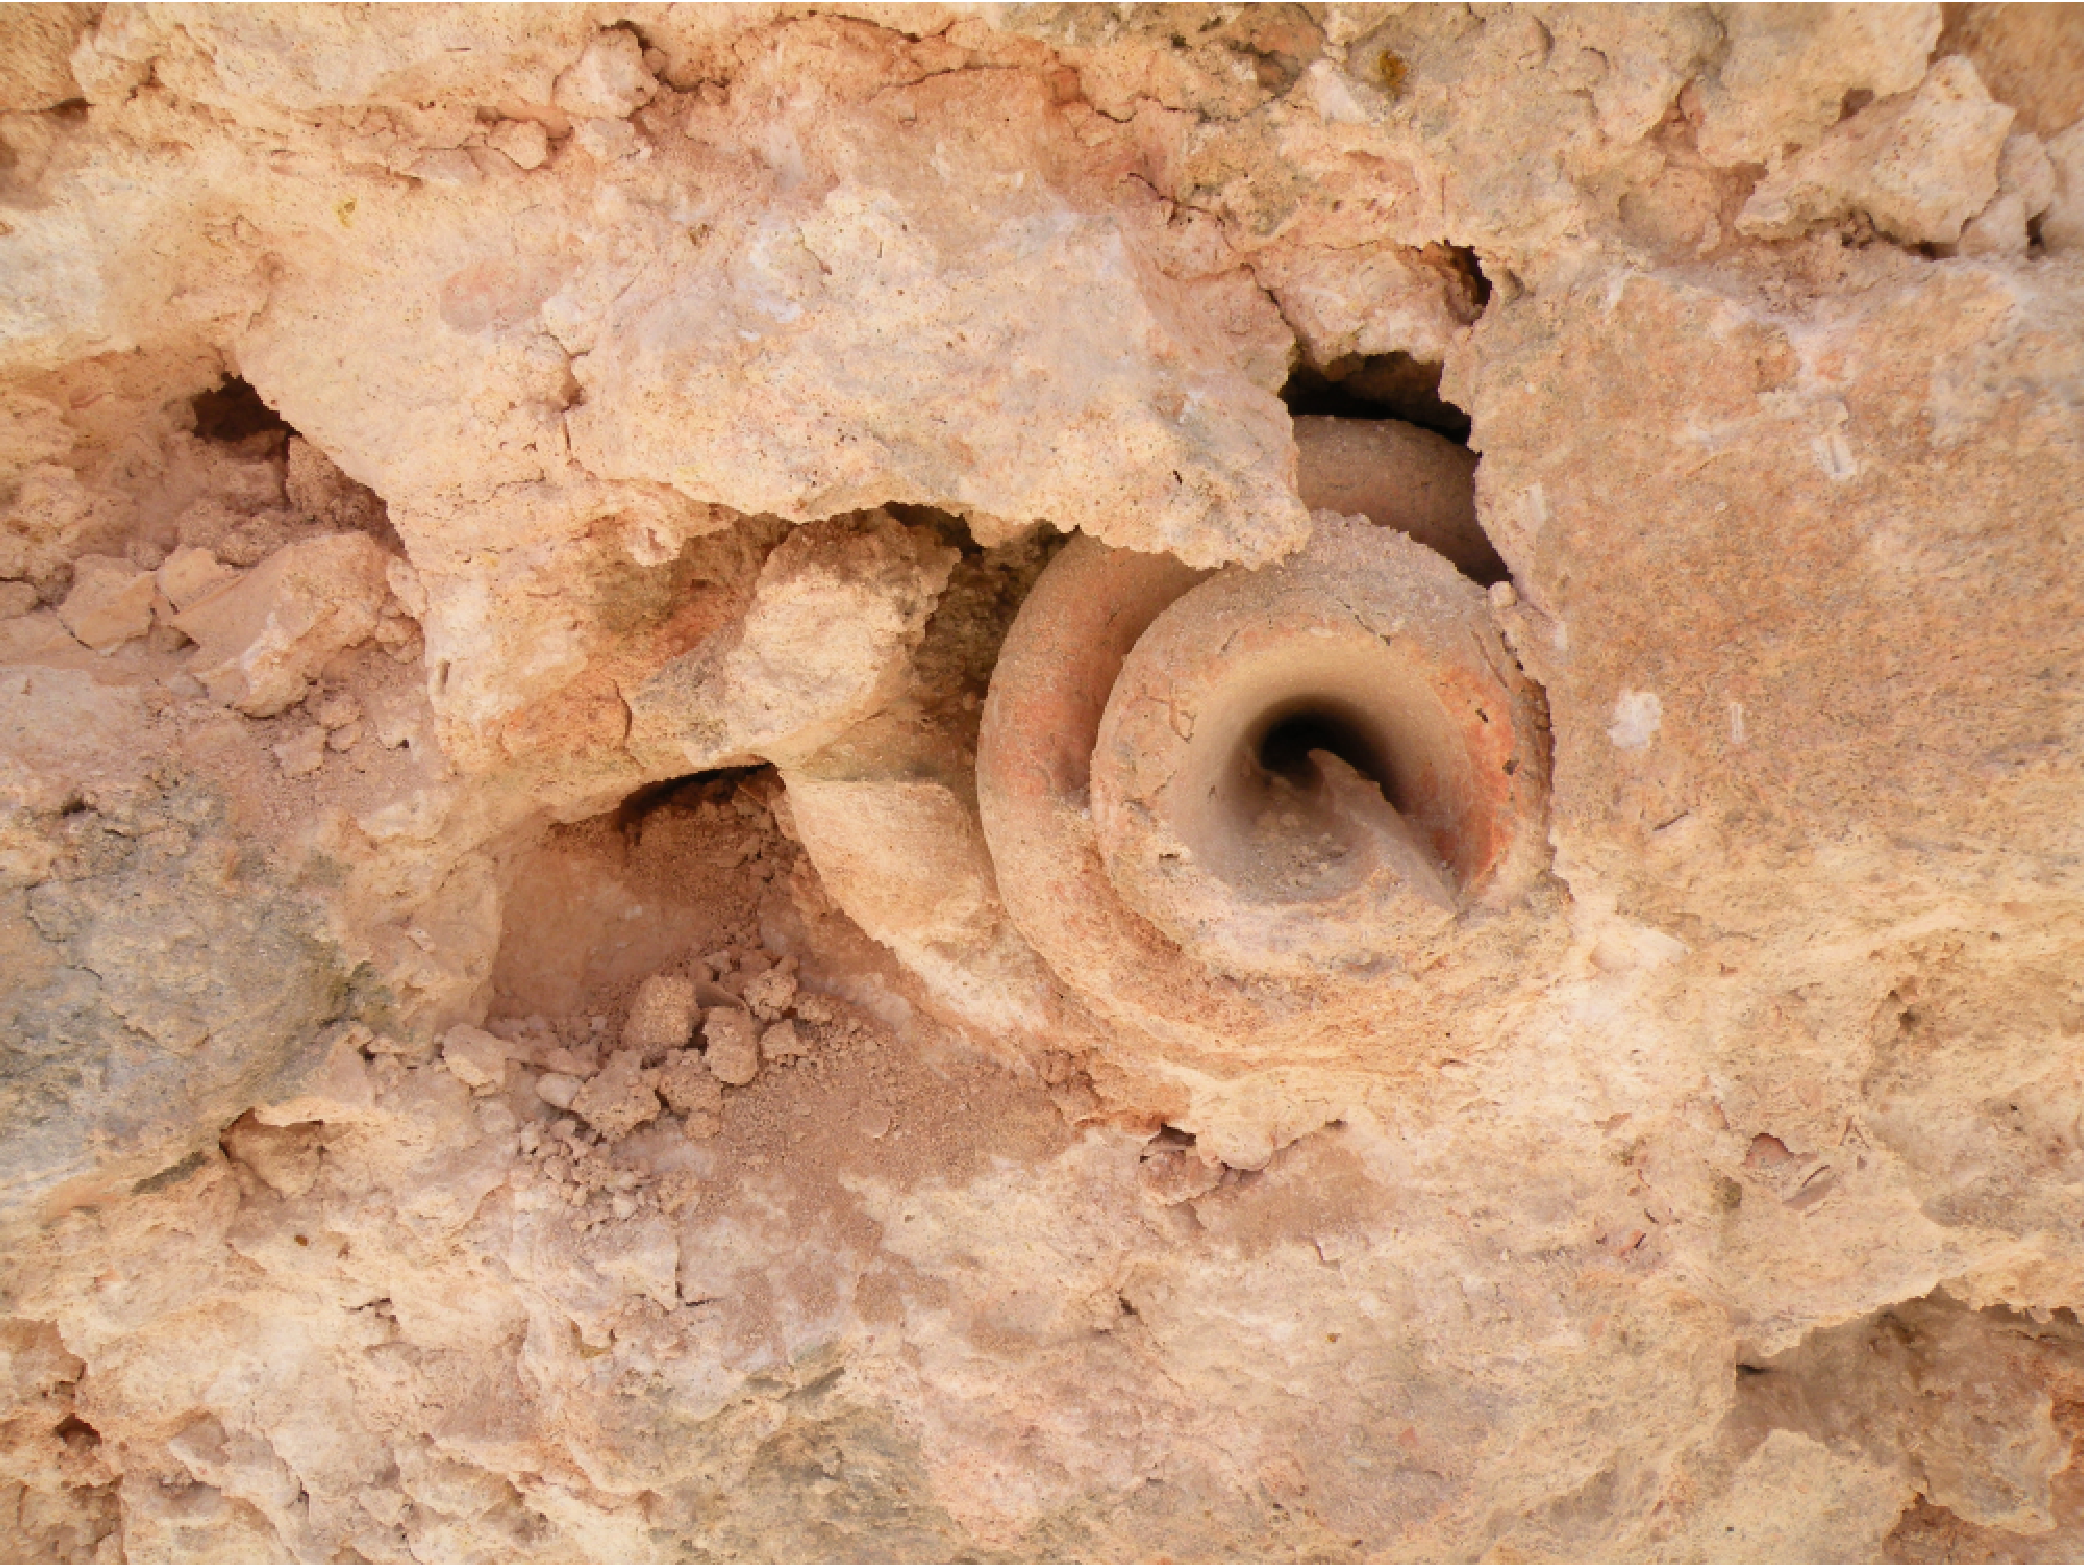
\includegraphics[width=10cm]{images/bsc-fossil}
    \end{center}
  \end{figure}
 % \vskip 2em%
\end{center}
  {\supervisor \\  \cosupervisor \\
  \flushright \year \par} 

\newpage
% If you have a photo on the titlepage, you can add a short
% explanataion here 
Cover photograph: Example of a fossil in a reef. Source: somewhere from the internet ...

\newpage

% Page numbering, options are arabic (Arabic numerals), roman	(Lowercase Roman), Roman (Uppercase Roman)
% alph (lowercase letters) and Alph (Uppercase letters)
\pagenumbering{Roman}
\pagestyle{plain}

% Include table of contents
\tableofcontents

% Remove the % in front of the command below to include a list of tables:
%\listoftables

% Remove the % in front of the command below to include a list of figures:
%\listoffigures

\newpage
% Use arabic numbering throughout the text
\pagenumbering{arabic}

% Include an abstract of your report
\abstract{

Place your abstract text here

} 



\section{Introduction}

The majority of flowering plants species depend on pollination by insects for reproduction. Any advantage in attractiveness can be crucial for the plants fitness in the competition for pollination service of a shared pollinator. However, the foraging behavior is complex and influenced by various factors \citep{goulson1999foraging}. One pattern affecting the flower decision of pollinators is frequency dependence. Generally, frequency dependence of survival or reproduction is defined as relative fitness of a species as a function of its frequency in the community \citep{ayala1974frequency,wright1946genetics}. In the case of plant-pollinator interactions, it occurs if the pollinator is influenced in its foraging behavior by the relative density of a species in a flowering community. Other species are neglected even if they are closer or more rewarding. Depending on their proportion in the flowering community, plants receive additional visits which can increase relative fitness and give an reproductive advantage due to increased seed set. According to ecological theory, frequency dependency can have far-ranging consequences for species coexistence and the maintenance of diversity \citep{levin1972low}. Two types of frequency dependence can be differenced: Negative frequency dependence describes the preference of pollinators for the rare flower types which can result in a stable polymorphic equilibrium and an increase in floral diversity \citep{gigord2001negative}. On the other hand, positive frequency dependence defines an advantage for the common phenotype which tends to reduce diversity in modeling studies (\citealt{may1974stability}, but see \citealt{bever1999dynamics}, \citealt{molofsky2002novel}). For animal-pollinated plant species, optimal foraging theory predicts that under most circumstances pollinators should favor common flower types over rarer ones \citep{kunin1996pollinator}.  \\

While the positive effect of density dependence for pollination success is well studied (e.g. \citealt{essenberg2012explaining,bernhardt2008effects,kunin1993sex,morris2010benefit}), frequency dependence has rarely been tested. However, the few previous studies of frequency dependent pollination cover laboratory, field and modeling experiments. \\
In the review by \cite{smithson2001pollinator}, 11 of 13 lab experiments using artificial flowers on a "bee-board" showed significant results for frequency dependence. 10 of those were done with rewarding flowers and resulted in positive frequency dependence favoring the abundant corolla color \citep{smithson1996frequency,smithson1997density}.  Negative frequency dependence was observed in the only experiment with non-rewarding flowers \citep{smithson1997negative}. \\
Field experiments on frequency dependence were either wholly or partly manipulative and concentrated on color morphisms. \cite{epperson1987frequency} found the rare white morph of \textit{Ipomoea purpurea} to be undervisited (but not the colored morphs) and \cite{gigord2001negative} proved negative frequency dependent selection for the rewardless orchid \textit{Dactylorhiza sambucina}, both supporting the lab experiments. However, \cite{Eckhart2006frequency} was the first to prove negative frequency dependence for a rewarding species (\textit{C. xantiana ssp. xantiana}) and to include natural frequencies. Other studies had no significant results (eg. \citealt{jones1996pollinator, mogford1978pollination}) and experiments on natural flower communities have not been conducted yet to our knowledge.\\
While foraging models are relatively common, few investigate frequency dependence. The game-theoretic model by \cite{kunin1996pollinator} suggests pollinators should favor common flower types over rarer ones when resource availability is high. The similar mathematical model of \cite{song2014adaptive} also concentrates on the pollinator perspective by applying rules of optimal foraging strategy to observe under which conditions the pollinators are able to maximize their net energy intake. Spatial explicit models grew in number over the last years addressing a range of foraging topics \citep{dornhaus2006benefits,bukovac2013bees,faruq2013biological}. Frequency dependent pollination is only subject to the model by \cite{hanoteaux2013effects} who tested survival strategies for less attractive species over multiple generations. \\
In summary, previous research on frequency dependence is limited and inconsistent between lab, field and simulation data. Rewarding flowers are underrepresented in field and lab experiments and studies of natural flower communities lack completely.  Furthermore, direct comparison of model and field data to cross-validate findings were only done for related questions such as density effects \citep{essenberg2012explaining} and the learning abilities of bees \citep{dyer2014bee} but never for frequency dependence.\\

Furthermore, little is known of the influencing factors on frequency dependence which can be responsible for differing results of previous research.  \cite{smithson2001pollinator} hypothesized in her review about factors including sampling size, floral traits and vision distance but did not test them. Density and spatial distribution of flowers can influence the perception of frequency of the pollinator and therefore also have interaction effects on frequency dependence.\\ 
While flower density is known to influence the foraging behavior of pollinators (eg. \citealt{kunin1993sex,essenberg2012explaining}), a possible interaction with frequency dependence was not considered in most cases. Exceptions were \cite{smithson1997density} who observed visitation rates for densities between 5 and 10\% in their lab experiment without any significant result. \cite{kunin1996pollinator} and \cite{song2014adaptive}  included density as factor in their mathematical model and found it strongly influencing the optimal foraging strategy of pollinators.\\

In contrast to habitat fragmentation, the influence of spatial structure and distribution of flowers is not well studied although flowers typically exist in patchy distributions of various levels and sizes. Flowers are often clustered in inflorescences which are again clustered on the plant itself. Also individual flowers are likely to be aggregated in patches over the meadow. Usually, the proportion of flowers visited by pollinators declines with increasing cluster size, probably due to limited memory structure and the avoidance of previously visited flowers \citep{goulson2000pollinators}. \cite{geslin2014effect} found the foraging behavior of bumble bees (\textit{Bombus terrestris}) affected by the spatial distribution of two co-flowering species in a controlled lab experiment. Again, the only study about spatial distribution of flowers in the context of frequency dependence was done by \cite{hanoteaux2013effects}. Within their model four levels of flower aggregation significantly influenced the survival rate of the less attractive species. The highest survival rates were found for big clusters in low frequencies and no clusters in high frequencies.\\ 

Given the general low quantity of studies concerning frequency dependent pollination and their inconsistent results, I want to address the following questions in this thesis:

\begin{enumerate}
	\item Does frequency dependent pollinator foraging exist for rewarding species in natural floral communities?
	\item	What kind of a frequency dependent relationship can be found?
	\item	What are important factors influencing frequency dependence?
\end{enumerate}

In a initial field study, I collected data on per-flower visitation rates of five different flowering rewarding plant species. Observations were made over a range of frequencies in their natural grassland plant communities in the area of the Jena Experiment. To understand which factors are influencing frequency dependence, I developed a spatially explicit model of two rewarding co-flowering plant species sharing pollination services. Agent-based models ("ABM", also known as individual-based models "IBM") are a valuable tool for assessing interactions in dynamic networks like financial markets, game theory, spread of diseases or, like in this case, ecosystems \citep{deangelis2005individual}. The model contains multiple agents which behave independently after given behavior rules and are able to interact with the environment and each other. Agent-based models are especially suitable for analyzing behavior shifts with changing environmental conditions. In the model, frequency, floral cover and cluster size were included in the main analysis to broaden the knowledge gained by the exploratory field study. This approach makes it possible to identify subsequent research options to further evaluate frequency dependence.

%The combination of an ABM with experimental data is a rare but promising approach. Fist to apply this method in foraging models was \citet{dyer2014bee}. They trained honey bees in a lab experiment to fine color discrimination to check for their flexibility to change when the reward changes between flower types. Afterwards, \citet{dyer2014bee} confirmed the findings with a ABM. 


%NOTES:
%
%+FDP
%- fixation on one phenotype for color morphs of one species
%- possible reduction of diversity (rare flowers do not get enough pollination, reproduction disadvantage) see Molofsky and Bever 2002
%- the most frequent species is becoming even more frequent
%
%reasons/explanations:
%- search image hypothesis (sensory system becomes trained, minimize search times)
%- search rate hypothesis (trade-off search time and probability to find the next rewarding flower)
%
%-FDS
%- promotes phenotye diversity
%- can promote landscape diversity
%- known for non-rewarding flowers
%
%reasons:
%- if a species is rare enough, the negative experience is not stored long enough in the short term memory and it gets exploratory vistits by the pollinator
%- naive pollinator hypothesis: non-rewarding species get visits from naive pollinators without knowledge to distinguish between rewarding and unrewarding species
%
%%%%%



%description other ABMs:
%\citet{dornhaus2006benefits} looked at the benefits of a recruitment system and colony sizes. \citet{faruq2013biological} compared the foraging success while applying different flower colors by varying the wavelengths over time. \citet{bukovac2013bees} simulated the difference between the parallel visual scan of honey bees and the serial visual scan of bumble bees to for the ability to avoid distractions during foraging. 

\label{ch:methods}

\section{Methods}

\subsection{Data Collection}

The Jena Experiment:

\begin{itemize}
\item N\ang{50;55;} E\ang{11;35;} ; 130 m a.s.l.
\item	Established in 2002
\item	Total Size: 10 hectars
\item	Arable field for 40 years before experiment started (therefore strongly fertilized)
\item	Plots are mowed every June and September
\item	Main experiment has 82 plots, each 20x20m (400m$^2$ )
\item	Originally sown species mix of 1,2,4,8,16 or 60 species, divided into four blocks (randomized complete block design) along abiotic gradients (mainly soil sand content)
\item	Part of the Plot is weeded twice a year (not my sampling area)
\end{itemize}


\subsubsection{Choosing Species and Plots}

The parts of the plots with continuous weeding were normally very scarce with flowers and had a very low species richness. So I collected the data in the “old invasion plots” (4m x 5.5m , 22m$^2$ ) and in the “new invasion plots” (5m x 3.5m, 17.5m$^2$ ) with a much higher cover, species richness and diversity. The "old invasion plots" were not weeded since the first seeding in 2002. The "new invasion plots" were not weeded since 2009.\\

I chose 5 species to observe (Those species were chosen because they were present in min. 5 plots with a differing frequency):

% Table generated by Excel2LaTeX from sheet 'Spec'
\begin{table}[htbp]
  \centering
  \caption{Focal Species}
    \begin{tabular}{rrrrrr}
    \toprule
    \textbf{Short} & \textbf{Name} & \textbf{German Name} & \textbf{Order} & \textbf{Family} & \textbf{Color} \\
    \midrule
    Ono   & Onobrychis viciifolia & Saat-Esparsette & Fabales & Fabaceae & pink+white \\
    Lat   & Lathyrus pratensis & Wiesen-Platterbse & Fabales & Fabaceae & Yellow \\
    Lot   & Lotus corniculatus & Gewöhnliche Hornklee & Fabales & Fabaceae & Yellow \\
    Ger   & Geranium pratense & Wiesen-Storchschnabel & Geraniales & Geraniaceae & Purple \\
    TP    & Trifolium pratense & Wiesen-Klee & Fabales & Fabaceae & Purple \\
    \bottomrule
    \end{tabular}%
  %\label{tab:addlabel}%
\end{table}%


Because the vegetation changed very quickly (heavy rain and very warm temperatures alternating) I chose max. 7 plots (= 14h) to observe at a time. 
Every time I finished a session I did a new sampling of all 82 plots of the Jena Experiment to check for suitable plots with focal plant species and their frequencies for the next round. Those observations were randomly distributed over the next days to prevent time dependencies ( observation times over the whole day for each plot)


\subsubsection{The Sampling}

\begin{itemize}
\item	Observations were made only during good weather conditions (max partly overcast, no rain, max light wind, min. 15 degree)
\item	Sampling time between 9am and 5pm (there was normally heavy fog and moist in the mornings so I could only start sampling from 10 or even 11)
\item	Sampling occurred between 20.7. -  12.8. 
\item Total of 15 sampling days (due to weather conditions)
\end{itemize}



\begin{figure}
\centering
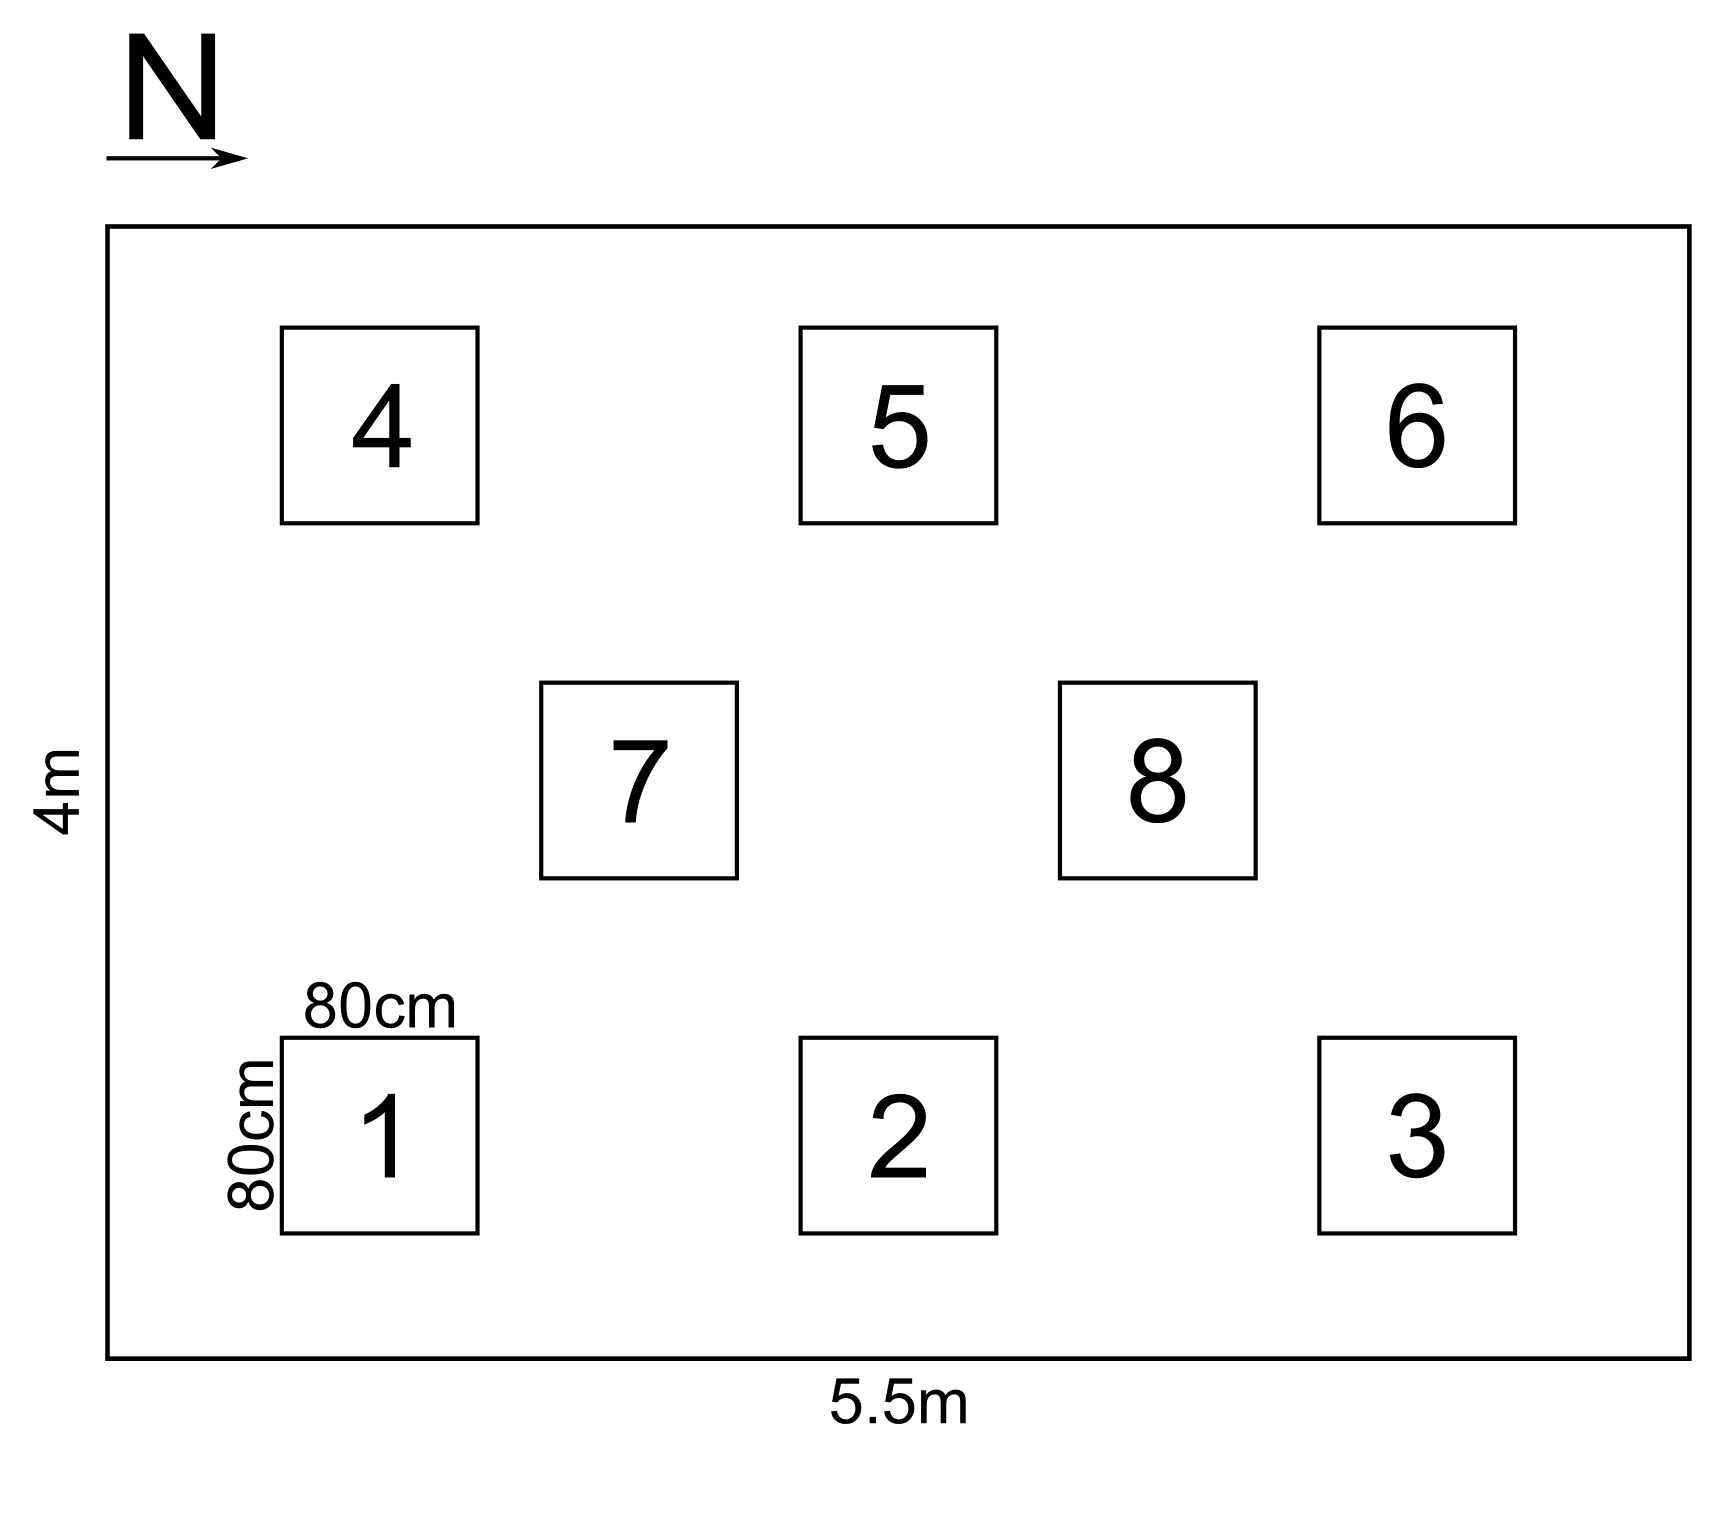
\includegraphics[width=9cm]{Images/plot-design}
 \caption{The sampling design within a plot}
 \label{fig:plot-design}
\end{figure}




\begin{itemize}
\item The pollinators were divided into bees, bumblebees, hoverflies and “other”
\item sampled eight of the 80x80cm patches per plot to get 2h of data per frequency and get a good mean over the plot (flowers were often in clusters and not distributed over the whole plot)
\item Patches were distributed as shown in Figure~\ref{fig:plot-design}
\end{itemize}

\begin{itemize}
\item When the flowers were very unevenly distributed over the Plot (which happened especially at low frequencies) I chose to observe some patches which contained flowers of the chosen species twice
\item I normally observed two species at once to save time/get a larger dataset. If there were not too many flowers that was easy feasible. If there were Plots with unevenly distributed flowers as explained above I observed the regular 1-8 patches for the evenly distributed species and additionally doubling patches for the uneven species. 
\item Eg. Geranium was flowering at all 8 patches, Lotus only in the southern part (patch 1,2,4,5, and 7). I regularly observed all patches 1-8 for Geranium. Because I was missing 3 patches for Lotus I doubled 1, 7 and 5. During this doubling I still kept track of visitors of the Geranium flowers. So in the end my dataset was the following:
\begin{itemize}
	\item 8+3 Geranium observations
	\item 8 Lotus observations
\end{itemize}
\end{itemize}


\subsection{Statistical Analysis}

\subsubsection{The Data}

Within the 4 weeks of sampling I got 386 entries, each equivalent to 15min of observation

\begin{itemize}
\item Flower visits to the focal species within the patch (divided by pollinator type)
\item Flower visits to other flowers except the focal species in the patch (divided by pollinator type)
\item Species Richness in the Patch (with names)
\item Species Richness in the Plot (with names and quantities)
\item Floral Cover in Patch and Plot (own estimation)
\item Frequency of the focal species in Patch and Plot
\item Count of individual flowers respectively inflorescence of the focal species
\item PlotID
\item PatchID
\item Date/Time
\end{itemize}


\subsection{The model}




  


\chapter{Results}

....das kommt dann noch irgendwann :)


\label{ch:discussion}
\section{Discussion}
Frequency dependence can influence the plants fitness and therefore have far reaching consequences for the development and maintenance of biodiversity. Aim of this thesis is to study the existence of frequency dependence in a natural plant community, explore the kind of relationship and identify the factors influencing frequency dependence with the help of an agent-based model.\\
I found evidence for frequency dependent pollination for rewarding flower species in grassland plant communities in the field data. The relationship is defined by a steep increase of visits within the first 20\% frequency followed by a disproportional low gain of visits for every additional flower due to an increase of frequency. When the species becomes dominant the per-flower visitation rate increases again. The combination of negative and positive frequency dependence combined in a cubic curve is generally supported by the agent-based model. Furthermore, the model reveals floral cover and cluster size as important influencing factors for frequency dependence. \\


Previous research found positive frequency dependence for lab experiments on rewarding flowers and inconsistence in the few field experiments focusing on color morphs \citep{smithson2001pollinator}. However, the field data shows a cubic pattern of frequency dependency for at least four different rewarding flower species and the results from the foraging simulation support the general shape of the per-flower visitation ratio. Where does the discrepancy of lab and field data comes from?\\ 

The sensitivity analysis of the agent-based model can give an explanation: If the reward function is increased to a refill within 10 time steps, the relationship is reversed to a positive frequency dependence and the rare species receives disproportionally few visits (Fig.~\ref{fig:SA_reward}). The curve is consistent with findings of  \cite{smithson1997density} and \cite{smithson1996frequency}. In their study design, artificial flowers were refilled after each foraging bout. Therefore, every bumble bee foraged on a set of full and equally rewarding flowers which is comparable to a high regrowth function in the agent-based model.\\
We know that pollinators more likely abandon flower constancy if they experience sequentially bad reward \citep{chittka1997foraging,goulson1994model}. If the reward is always high, pollinators have less incentive to go on exploratory visits to the rare species as the abundant type is easy to find and sufficient rewarding. Hence it can be assumed that negative frequency dependent selection does not exclusively apply for non-rewarding species but also for flowering communities with varying or insufficient reward. Strong positive frequency dependence in pollination might be only possible for highly rewarding or artificial systems. 

%More research, especially on natural field conditions, is needed to confirm this hypothesis.

%high nectar production rates increases approach rates Pleasants 1981; Real & Rathcke 1991;Duffield al 1993; Shykoff & Bucheli 1995 (from  Klinkhamer 2001)

\subsubsection*{Floral cover and cluster size are influencing factors}
The model reveals two main influences for frequency dependence: The higher the floral cover, the stronger the frequency dependence and the bigger the clusters, the weaker the frequency dependence (Fig.~\ref{fig:PFV}e-h). 
Floral density is known to influence visitation rates, usually positive and with a saturating function (eg. \citealt{rathcke1983competition,essenberg2012explaining,bernhardt2008effects,Kunin1997}). Those findings are consistent with the Holling´s type II functional response found for different cover values (Supplementary material, Fig.~\ref{fig:nonfreq}a). If the cover is increasing, the absolute number of flowers rises also for the rare species. That makes it more likely for a bee-agent to find a flower before changing preference towards the common species due to long search times even if foraging on the later would be more efficient. Therefore, high cover causes the same effect as expanded vision distance or maximum search limit (cf. Fig.~\ref{fig:SA_view} and Fig.~\ref{fig:SA_flight}): The main reason of abandoning flower constancy becomes multiple visit of flowers with low reward. Consequence are explanatory visits to the rare species which can have a great impact on the per-flower visitation rate. Every visit to a rare species weights high in the per-flower visitation rate because the sum of visits is divided through the number of flowers.\\ 

The model shows that spatial aggregation of flowers can lead to a more efficient foraging (more visits per time unit), less frequency dependence and a higher quality of visits due to compatible pollen deposits. If flowers are randomly distributed over the whole meadow, many short search and flight times apply. An intermediate cluster level is easy to exploit by a pollinator whereas the flight and search times can be very long in between few big clusters, especially for low floral densities. \\
It was already suggested by \cite{epperson1987frequency} that spatial agglomeration of flowers decreases frequency dependence. In the agent-based model, a similar effect compared to low cover takes place: If flowers are aggregated at few places, they affect the pollinators perception of frequency and are more difficult to find. Long search times will weaken the bee-agents flower preference and lead to foraging on the next available cluster independent of its species. 

%more literature!

\subsubsection*{Requirements for successful pollination}
High visitation rate is gained at low frequency with high cover and low cluster size. However, those visits might not be the best quality if the pollination per visit ratio is comparatively low (Fig.~\ref{fig:POC}a,d). The ratio can be seen as index for flower constancy: If the majority of visits lead even for a small pollen carryover value to successful pollination the bee-agents forage very flower constant \citep{montgomery2009pollen}. If the cover is high, bee-agents will keep their constancy also for rare species because they are abundant enough. If the aggregation of flowers is high, bee-agents exploit this cluster before leaving for the next. Every visit within a cluster of flowers of the same species is counted as successful pollination and can lead to a high visit quality even if the cover is low (cf. \citealt{jakobsson2009relationships}). Therefore, rare species should occur in clusters of flowers if the cover is low to get a maximum of pollination per visit. If the cover is high the spatial distribution plays a minor role for the visit quality.  

%vgl Hanoteux?
%see Feldmann 2008

\subsubsection*{Sum of visits to the flower community also show frequency dependence}
Additionally to individual frequency dependence, I analyzed the impact of species partitioning on frequency dependent visitation in the system as whole. \\
If the cover is very low, a maximum in total visits can be received if one species is dominant. Co-flowering will lead to longer search times and less overall visits (u-shape for 5\% cover in Fig.~\ref{fig:SUM}a). For higher cover, the frequency dependence shows a function similar to a fourth-degree polynomial. If one species is rare at 5-20\% frequency, pollinators exhibit exploratory visits to the rare species and spend inefficient time searching. Hence, the total visitation number drops to a minimum. If species are evenly distributed the pollinators forage on both species in equal amounts. This is the most efficient status for the overall ecosystem, especially for high cover or cluster size. \\
Spatial aggregation weakens the frequency effect but will also reduce the total visits. If flowers are even and random distributed, the bee-agent has many small search times intermittent by collecting reward on a single flower and continue foraging. Rare flowers can be found comparatively easy if they are spread over the whole meadow and flower constancy will be kept even if it is highly inefficient. If the clusters of flowers are bigger, bee-agents will not find rare flowers that easily because they might occur only in a single cluster on the meadow. The bee-agent switches to the common flower, the minimum at very uneven distribution disappears and the relationship becomes slightly hump-shaped (Fig.~\ref{fig:SUM}b,c). \\
A maximum of overall visits favoring both the pollinators and the co-flowering plants can be achieved with balanced abundance in high cover and very uneven species distribution for low floral cover environments. 

\subsubsection*{Limitations of the study design and research suggestions}
Even though modeling can be an excellent tool to understand and interpret ecological data, some questions evolve comparing the data collected in the Jena Experiment and the foraging model. Floral cover is an important factor in the outcome of the model. It influences not only the absolute number of visits but also the intensity of frequency dependence. But it was removed in the model selection as it was no factor of explanatory power to the per-flower visitation data. 
Reason could lie in the sampling design. Data was only observed from plots with an intermediate cover, no extremes were taken into account. In total, there were only five values for cover in the final analysis. Also all cover values are estimations, no exact measurements. Also, pollinators are influences by many factors in the field, not all of them measured in this study or possible to take into account at all. Other floral traits like scent, the pollinators detection of colors and differences in pollinator types are just some factors which might have an impact on the foraging behavior and consequently also on frequency dependence. \citep{smithson2001pollinator}. \\

Validation of further results of the agent-based model can be made via a supplementary study with varying frequency, cover and cluster size of two co-flowering species. Practical is a simplified study design with less influencing variables either under natural conditions where manipulation is possible (eg. \citealt{Eckhart2006frequency,essenberg2012explaining}) or with potted plants \citep{epperson1987frequency}. Also results of the frequency dependent sum of visits could be tested by manipulated field experiments. Natural conditions data are not suitable for this purpose because every plot contains more than two co-flowering species with unequal attractiveness.  
The data collected in Jena shows drastic differences in attractiveness of the focal species and frequency dependence was found to be subject to each species. Therefore I suggest continuous research on a variety of species, both rewarding and unrewarding with measurements of reward to check if my findings are universally valid.\\


\chapter*{Acknowledgements}
\label{ch:Acknowledgements}
\addcontentsline{toc}{chapter}{Acknowledgements}

And of course include your acknowledgements here: my supervisor was always there for me, taught me so much and hence will receive eternal praise and gratefulness. Actually, I rarely saw him/her and that was just as well.



   
% Insert the references
\bibliographystyle{plainnat}
\bibliography{library/studlib}

% Anything behind this command will be treated as an appendix
\appendix

% Insert the first appendix
\chapter{This is Appendix 1...}
\label{app:appendix1}

Put appendix text here


% Insert the second appendix

% insert a second appendix
\chapter{This is appendix 2...}
\label{app:appendix2}

Put appendix text here...




% If you used the makeidx package to create an index then use the 
% following command to print the index
\printindex

\chapter*{Selbstständigkeitserklärung} % (in German!)

\vspace{2cm}

\section*{Erklärung}

Ich versichere hiermit, dass ich die vorliegende Arbeit ohne fremde Hilfe selbstständig verfasst und nur die angegebenen Quellen und Hilfsmittel benutzt habe. Wörtlich oder dem Sinn nach aus anderen Werken entnommene Stellen habe ich unter Angabe der Quellen kenntlich gemacht.

\medskip
\noindent (I hereby declare that I have composed this document unassistedly and that I only used the sources and devices I declared. Passages taken verbatim or in meaning from other sources are identified as such and the sources are acknowledged and cited.)

\vspace{2cm}

\noindent \year

\end{document}